\documentclass[aps,prd,onecolumn,superscriptaddress,nofootinbib,floatfix]{revtex4-2}
\usepackage{amsmath,amssymb}
\usepackage{graphicx}
% ragged-right table cells (array.sty clashes with REVTeX)
\newcommand{\RR}{\raggedright\let\\\tabularnewline}
\usepackage[colorlinks=true,allcolors=blue]{hyperref}

\newcommand{\fpbh}{f_{\rm PBH}}
\newcommand{\Msun}{M_\odot}
\newcommand{\Treh}{T_{\rm reh}}
\newcommand{\wreh}{w_{\rm reh}}
\newcommand{\Ns}{N_\ast}
\newcommand{\code}[1]{\texttt{#1}}
% references to the paper
\newcommand{\Pap}{the paper}

\begin{document}
\sloppy

\title{Analysis notes for ``Where primordial black holes can come from:\\ how likely formation mechanisms are to produce a given mass and abundance''}

\author{Tomohiro Matsuda}
\affiliation{Saitama Institute of Technology}

\date{\today}

\begin{abstract}
These notes accompany the code that produces every figure and number of the paper named in the title (``the paper'' below). They give, for each formation mechanism, the map from parameters to the mass function, the parameter ranges and the conditions that define the allowed region; the external data; the statistical procedures; the construction of each figure; analytic estimates that check the numerical results; and the commands that reproduce them. Physical motivation is given in the paper and is not repeated. Equation, figure, table and section numbers of the paper are written as, e.g., ``Eq.~(1) of the paper''.
\end{abstract}

\maketitle

%=======================================================================
\section{Conventions and map of the code}\label{sec:conv}

\paragraph*{Notation.}
The supercooled first-order phase transition is abbreviated as FOPT, the inflaton potential with a small Gaussian bump as the inflaton bump, and domain walls as DW. $p_c$ is the probability that a mechanism produces PBHs in square $c$ of the plane without violating a current PBH limit [Eq.~(1) of the paper]. The plane is $\log_{10}(M/\Msun)\in[-18,6]$, $\log_{10}\fpbh\in[-12,0]$, divided into squares one third of a decade wide. A \emph{treatment} is one of the theoretical variants of a mechanism (for example a collapse threshold or a value of $L/t$); the treatments that enter the optimistic and conservative columns are listed in Sec.~V of the paper. A \emph{condition} in the code is a stored result for one mechanism and one treatment. $R$ is the region of parameter space allowed by the non-PBH observations, $B$ the parameter range (box) in which $R$ is searched, and the parameter distribution is the Gaussian with the mean and covariance of a uniform distribution over $R$, set to zero outside $R$ [Eq.~(2) of the paper]. Logarithms are to base ten unless written $\ln$; temperatures are in GeV.

\paragraph*{Code.}
The repository is \url{https://github.com/Tomohiro-Matsuda-SIT/pbh-formation-map}. All code is in the directory \code{pbh/}; Table~\ref{tab:code} lists which file implements which part. File locations are collected in \code{paths.py}, and each mechanism module states its assumptions in its header. The Markdown file \code{AI\_GUIDE.md} at the top of the repository describes the same structure in a form intended for AI assistants, together with the interface a new mechanism must provide.

\begin{table}[htbp]
\caption{Where each part of the analysis is implemented (directory \code{pbh/}).}
\label{tab:code}
\begin{ruledtabular}
\begin{tabular}{p{5.2cm}p{11.0cm}}
\RR Part & \RR Files \\
\hline
\RR Grid, limit curves, result store, per-result figures & \RR \code{results\_store.py} \\
\RR Extended mass functions, PBH limits & \RR \code{emf.py} (current and planned limits), \code{evap.py} (evaporated PBHs) \\
\RR Degrees of freedom; reference inflation model & \RR \code{gstar\_ss.py}; \code{curvaton\_pipeline.py} (Starobinsky background and conversion tables) \\
\RR $\alpha$-attractor family & \RR \code{background.py}, \code{bg\_prior.py}, \code{bg\_run.py}, \code{bg\_node.py}, \code{bg\_combine.py}; ACT-compatible members: \code{bg\_prior\_act.py}, \code{bg\_act\_combine.py} \\
\RR Quadratic curvaton & \RR \code{curvaton\_pipeline.py} \\
\RR Axion-like curvaton & \RR \code{axion\_G.py}, \code{axion\_pipeline.py}, \code{axion\_zc.py} (threshold), \code{axion\_target\_de.py} (targeted search) \\
\RR Inflating curvaton & \RR \code{infcurv\_pipeline.py}, \code{infcurv\_opt\_de.py} (global maximization) \\
\RR FOPT and DW & \RR \code{fopt\_dw\_pipeline.py}, \code{dw\_pta\_fit.py}, \code{run\_dw\_ptaL.py}, \code{patch\_dw\_width.py}, \code{fopt\_gwvar.py} (GW spectra), \code{dw\_bayes.py} (Bayes factors) \\
\RR Fermi balls & \RR \code{fermiball\_pipeline.py} \\
\RR Walls from inflation; string loops & \RR \code{infwall\_pipeline.py}, \code{infwall\_reh.py}; \code{cosmicstring\_pipeline.py} \\
\RR Inflaton bump & \RR \code{usr\_solver.py}, \code{usr\_pbh.py}, \code{usr\_pipeline.py}, \code{usr\_pushforward.py}, \code{usr\_prior\_sens.py} \\
\RR PTA likelihood & \RR \code{pta\_like.py} \\
\RR Building the result store & \RR \code{build\_results.py} \\
\RR Figures and variations & \RR \code{fig\_combined.py} (classes), \code{measure\_checks.py}, \code{measure\_plots.py} (maximum probability per square, threshold curves, uniform distribution, square size), \code{robustness.py} (variations, square-by-square summary), \code{paper\_figs.py} \\
\RR Analytic estimates & \RR \code{analytic.py} \\
\RR Reproduction & \RR \code{regenerate.py} (Sec.~\ref{sec:repro}) \\
\end{tabular}
\end{ruledtabular}
\end{table}

%=======================================================================
\section{Pipeline and external inputs}\label{sec:inputs}

Each figure is built in four steps. (1) For a mechanism and a treatment, the allowed region $R$ and the parameter distribution are constructed. (2) Samples are mapped to $(M_\ast,\fpbh)$, where $M_\ast$ is the peak of the mass function, and flagged by $\mathbf{1}_{\rm ok}$ (current limits, including limits on evaporated PBHs) and by detectability (planned limits). (3) The samples are stored per treatment in \code{results/<mechanism>/<condition>/} and histogrammed into $p_c$. (4) The figures combine stored treatments only; no figure recomputes a mechanism. Table~\ref{tab:inputs} lists the external inputs.

\begin{table}[htbp]
\caption{External data and fixed inputs.}
\label{tab:inputs}
\begin{ruledtabular}
\begin{tabular}{p{3.4cm}p{12.8cm}}
\RR Input & \RR Value / source \\
\hline
\RR Cosmology & \RR $A_s=2.1\times10^{-9}$ at $k_\ast=0.05\,{\rm Mpc}^{-1}$; $\Omega_{\rm DM}h^2=0.120$, $h=0.674$~\cite{Planck:2018jri} \\
\RR CMB bands & \RR $n_s=0.9649\pm0.0042$, $\alpha_s=-0.0045\pm0.0067$~\cite{Planck:2018jri}; $n_s=0.9743\pm0.0034$~\cite{AtacamaCosmologyTelescope:2025blo}; $r<0.036$~\cite{BICEP:2021xfz}; all applied at two standard deviations \\
\RR $g_\rho(T)$, $g_s(T)$ & \RR fitting functions of Ref.~\cite{Saikawa:2018rcs}, App.~C \\
\RR Current PBH limits & \RR PBHbounds~\cite{PBHbounds} (commit 96bc091), files Evaporation, Microlensing, GWs, Accretion, Dynamical \\
\RR Planned limits & \RR PBHbounds: 3G-GW-10y, GECCO, Xraylensing-Xmu-proj, Xraylensing-eXTP-proj, WhiteDwarfmicro, PTA-Doppler, PTA-Shapiro, SKA, GRB-parallax, FL-small \\
\RR Evaporated PBHs & \RR BBN~\cite{Kohri:1999ex}; CMB distortions, anisotropies, extragalactic gamma rays and the general limit $\beta'<10^{-18}$~\cite{Carr:2020gox}; conversion to the would-be present abundance~\cite{Carr:2009jm} \\
\RR LVK & \RR $\Omega_{\rm GW}<5.8\times10^{-9}$, 20--76.6\,Hz, applied at 25 logarithmically spaced frequencies~\cite{KAGRA:2021kbb} \\
\RR PTA & \RR NANOGrav 15-year Hellings--Downs free spectrum, first 14 bins, kernel-density representation~\cite{NG15KDE,Lamb:2023jls} (Zenodo 10.5281/zenodo.10344086, v1.0.0); EPTA DR2 (9 bins) for comparison~\cite{EPTA:2023fyk} (ceffyl data, commit 0cd2b3a) \\
\RR Cosmic strings & \RR $G\mu<4\times10^{-15}$~\cite{LIGOScientific:2021nrg} \\
\end{tabular}
\end{ruledtabular}
\end{table}

The limit $f^{\max}_k(M)$ of group $k$ is the pointwise minimum of the curves in that group, interpolated linearly in $(\log M,\log f)$ and evaluated at the square centres; outside the mass range of a curve that curve imposes no limit. A sample with mass function $\psi$ passes group $k$ if $\int d\ln M\,\psi/f^{\max}_k\le1$~\cite{Carr:2017jsz} [Eq.~(3) of the paper]. Horizon mass, comoving scale and present abundance are related through
\begin{align}
M&=\gamma\,\frac{4\pi M_P^2}{H(T)},\qquad \frac{\fpbh}{\beta}=\frac{\rho(T)\,a^3(T)}{\rho_{\rm DM,0}\,a_0^3},
\label{eq:conv}
\end{align}
with $\gamma=0.2$ unless a mechanism specifies its own mass, $\rho=\frac{\pi^2}{30}g_\rho T^4$ and $a\propto g_s^{-1/3}T^{-1}$. Here $\beta$ is the mass fraction of the Universe in PBHs at formation.

%=======================================================================
\section{Mechanisms: maps, ranges and constraints}\label{sec:mech}

Table~\ref{tab:boxes} gives the parameters and ranges.

\begin{table}[htbp]
\caption{Parameters and ranges $B$. Edges marked $\dagger$ are theory choices varied in Sec.~VI of the paper.}
\label{tab:boxes}
\begin{ruledtabular}
\begin{tabular}{p{3.2cm}p{13.0cm}}
\RR Mechanism & \RR Parameters and ranges \\
\hline
\RR Quadratic curvaton & \RR $m/H_\ast\in[0.05,1.5]$, $\log\sigma_\ast/H_\ast\in[-1,7]$, $\log T_{\rm dec}\in[\log5\times10^{-3},\log\Treh]$ \\
\RR Axion-like curvaton & \RR $c\in[0.2,2.2]$, $N_f\in[0,\Ns-5]$, $\log f_a/H_\ast\in[-1,5]$, $\theta_i\in[0.01,\pi-10^{-3}]$, $\log m\in[-20,\log0.1H_{\rm end}]$, $\log T_{\rm dec}$ as above \\
\RR Inflating curvaton & \RR $c_1$, $\log\sigma_\ast/H_\ast$, $\log T_2$, $\log\eta_2$, $\log\sigma_{\rm end}/M_P$ (maximization of $\fpbh$ over $R$) \\
\RR FOPT & \RR $\log T_{\rm eq}\in[\log5\times10^{-3},\log\Treh]$, $\beta/H\in[3,30^\dagger]$ \\
\RR DW & \RR $\log T_{\rm ann}\in[\log5\times10^{-3},9]$, $\log\alpha_{\rm ann}\in[-4^\dagger,0]$ \\
\RR Fermi balls & \RR $\log T_\ast\in[\log5\times10^{-3},\log\Treh]$, $\log\beta/H\in[1,4]$, $\log\alpha\in[-2,1]$, $\log\eta_\chi\in[-16^\dagger,-6]$ \\
\RR Walls from inflation & \RR $x=\log\sigma^{1/3}/H_\ast\in[x_{\min}(A),\log M_P^\dagger/H_\ast]$ \\
\RR String loops & \RR $\log G\mu\in[-26^\dagger,\log\min(G\mu_{T_{\max}},4\times10^{-15})]$, $\log f\in[-30,0]$ \\
\RR Inflaton bump & \RR $\phi_0\in[2.9,5.1]$, $\log s\in[-2.3,-1.3]$, $\log A\in[-6,-1]$ \\
\end{tabular}
\end{ruledtabular}
\end{table}

\paragraph*{Quadratic curvaton.}
During inflation $\ln\sigma$ decreases at the rate $\lambda(N)=\frac32[1-(1-4m^2/9H(N)^2)^{1/2}]$ per $e$-fold; a mode exiting at $N_k$ has $\mathcal{P}_x=(H_k/2\pi\sigma_k)^2$, $x=\delta\sigma/\sigma$. The energy fraction at the onset of oscillations is $\Omega_{\rm osc}=\sigma_{\rm end}^2/6M_P^2$ and grows as $a$ until decay, $p=\Omega_{\rm osc}[g_s(\Treh)/g_s(T_{\rm dec})]^{1/3}\Treh/T_{\rm dec}$, $\Omega_{\rm dec}=p/(1+p)$. The curvature perturbation follows from $(1-\Omega_{\rm dec})e^{-4\zeta}+\Omega_{\rm dec}(1+x)^2e^{-3\zeta}=1$~\cite{Sasaki:2006kq}, with $x$ Gaussian. PBHs form where $\zeta>\zeta_c$ ($\zeta_c=0.7,1.0,1.3$), which is evaluated as a threshold $x>x_c(\zeta_c,\Omega_{\rm dec})$ on the Gaussian variable; the variance is smoothed with $e^{-q^2/k^2}$ and only $k\le k_{\rm dec}$ contributes. The constraints are: curvaton contribution to $A_s$ below 1\% and $|f_{\rm NL}|<5$; $m<\frac32H$ throughout; spectator energy below 1\%; $\mathcal{P}_x<1$ on all scales; $5\times10^{-3}<T_{\rm dec}<\Treh$.

\paragraph*{Axion-like curvaton.}
The radial field decreases as $\phi\propto e^{\lambda_\phi(N-N_f)}$ for $N>N_f$, giving $\mathcal{P}_{\delta\theta}=(H/2\pi\phi)^2$. The anharmonic energy fraction uses $\Omega=(f_a/M_P)^2G(\theta)\times$[growth factor of the matter- or radiation-dominated era in which oscillations start], with $G(\theta)$ computed numerically and fitted near the hilltop by $G^{1/2}=1.412u+2.636$ (matter era) and $G^{2/3}=2.283u+3.049$ (radiation era), $u=-\ln(\pi-\theta)$. The constraints add: no crossing of the hilltop at $1\sigma$, and perturbative decay $H(T_{\rm dec})<m^3/16\pi f_a^2$. ``Optimistic'' counts realizations within the sub-scale fluctuation of the hilltop; ``conservative'' excludes them.

For the targeted search of Sec.~IV\,A of the paper, $\log_{10}\fpbh$ is maximized by differential evolution (population 120, 150 generations, up to three seeds) over the six parameters $(c,N_f,\log f_a/H_\ast,\theta_i,\log m,\log T_{\rm dec})$, with the peak mass required to lie within half a decade of the target and with a penalty that keeps the population inside $R$; the search is repeated with each of the four groups of conditions (CMB, light spectator, no hilltop crossing, decay) removed in turn. For targets of $10^{-13}$, $10^{-9}$, $10^{-4}$, $1$ and $10^{1.5}\,\Msun$ the largest values found are $\log_{10}\fpbh=-9.1$ (optimistic), $+2.2$ (optimistic), $-114$ (conservative), $-0.1$ and $+1.2$ (both conservative). The optimizer does not converge reliably on this function, whose value changes by thousands of decades across $R$; a repetition with a different penalty returned lower values for the two heaviest targets. The numbers are therefore lower limits on the maxima. The best points are stored in \code{axion\_target\_best.json}.

\paragraph*{Inflating curvaton.}
A vacuum energy $V_0=\rho_r(T_2)$ drives $N_2=\ln(\sigma_{\rm end}/\sigma_{\rm ini})/g_2$ $e$-folds with $g_2=\frac32[(1+4\eta_2/3)^{1/2}-1]$; $\zeta=r\zeta_\sigma$, $\zeta_\sigma=-g_2^{-1}\ln|1+x|$, $r=[1+\frac43e^{-4N_2}]^{-1}$; $\Ns$ and $\mu$ are re-solved for every $N_2$. Because no sample of $R$ gives $\fpbh>10^{-12}$, the largest abundance is found by differential evolution over $R$ (population 200, 400 generations, four independent seeds that converge to the same maximum), with a penalty proportional to the logarithmic violation of each constraint outside $R$. Searches with 797 and $3\times10^4$ points drawn uniformly in $R$ return much lower maxima ($\log_{10}\fpbh\lesssim-2.4\times10^{5}$), because the maximum lies in a corner of $R$ ($\eta_2\simeq0.75$, $N_2=1$, $T_2\simeq\Treh$). The constraint $|f_{\rm NL}|<5$ uses the value $f_{\rm NL}=\frac56g_2/r$ that follows from the logarithmic map; the expansion of Ref.~\cite{Enomoto:2012uy} gives $f_{\rm NL}\simeq\frac52\eta_2$ for $r=1$ and a quadratic potential, a factor of about three larger. Since $\eta_2<\frac34$, both satisfy the constraint, and the choice does not affect the result. The checks of Sec.~IV\,A of the paper repeat the maximization with $\zeta_c=0.5$; without the $n_s$ constraint and with $N_2\le30$; additionally without $\mathcal{P}_x<1$ at the end of the first inflation; without $\sigma_\ast<M_P$ and the spectator-energy bound; and with the Hubble rate of the first inflation scaled down to $2.4\times10^{11}$\,GeV (CMB perturbations from another source, curvaton contribution still below 1\% of $A_s$). Over all masses, including evaporated black holes, the maxima are $-3.8\times10^{3}$ (reference constraints), $-1.3\times10^{3}$, $-3.8\times10^{3}$, $-3.8\times10^{3}$, $+18$ and $+18$. Restricted to $M>5\times10^{14}$\,g they are $-7.0\times10^{3}$ for the reference constraints and $+17$ for the low Hubble rate.

\paragraph*{FOPT.}
Non-covariant treatment~\cite{Gouttenoire:2023naa}: $P_{\rm coll}=\exp[-1.024\,(\beta/H)^{0.6921}(1+\delta_c)^{0.8831\beta/H}]$, $\fpbh=(P_{\rm coll}/2.2\times10^{-8})(T_{\rm eq}/140\,{\rm MeV})$, $M_H=\Msun(20/g_\ast)^{1/2}(140\,{\rm MeV}/T_{\rm eq})^2$. The mass function follows from critical scaling, $M=\mathcal{K}M_H\Delta^{\gamma}$ with $\mathcal{K}=3$ and $\gamma=0.36$, and $\Delta$ exponentially distributed with scale $s=-(d\ln P_{\rm coll}/d\delta_c)^{-1}$; its peak is $M_\ast=\mathcal{K}M_H[(1+\gamma)s]^{\gamma}$. Covariant treatment~\cite{Franciolini:2025ztf}: the density-contrast distribution of their Eq.~(24) with the parameters of their Table~I interpolated in $\ln\beta/H$, $\beta=P_0\int_{\delta_c}P\,d\delta$ by a Laplace estimate, $\fpbh\simeq(\beta/10^{-10})(T/{\rm GeV})$ and $M_k=4.8\times10^{-2}\Msun(106.75/g_\ast)^{1/2}({\rm GeV}/T)^2$. GWs: envelope approximation, $h^2\Omega=1.67\times10^{-5}(H/\beta)^2(100/g_s)^{1/3}(0.11/1.42)S_{\rm env}$, $S_{\rm env}=3.8x^{2.8}/(1+2.8x^{3.8})$, $x=f/f_{\rm env}$, $f_{\rm env}=16.5\,\mu{\rm Hz}\,(0.62/2.7)(\beta/H)(T/100\,{\rm GeV})(g_s/100)^{1/6}$~\cite{Caprini:2015zlo}. The alternative spectra of Sec.~\ref{sec:fopt-gw} are selected with the environment variable \code{PBH\_FOPT\_GW}.

\paragraph*{Domain walls.}
With $L=\log_{10}\alpha_{\rm ann}$: $t_{\rm dom}=t_{\rm ann}/\sqrt{3\alpha_{\rm ann}}$, $R/t_{\rm ann}=0.780L^2-0.618L+0.407$, $r=(R/t)/(L/t)$, $s_{\rm ball}/r^3=8+\frac12[1+\tanh(1.15\ln(r/5.55))](\frac{4\pi}3-8)$, $\fpbh=(T_{\rm dom}/{\rm TeV})\,s_{\rm ball}p^{s_{\rm ball}}/8\times10^{-13}$ with $p=0.5$, $M=4\pi M_P^2t_{\rm dom}$, and tension $\sigma=3\alpha_{\rm ann}M_P^2/(4\mathcal{A}t_{\rm ann})$, $\mathcal{A}=0.8$~\cite{Gouttenoire:2023ftk,Gouttenoire:2023gbn}. GWs: $h^2\Omega=D\frac{3}{32\pi}\,0.7\,\alpha_{\rm ann}^2\,2/[(f/f_p)+(f_p/f)^3]$, $D=3.49\times10^{-5}(g_\ast/10.75)(10.75/g_s)^{4/3}$, $f_p=1.08\,{\rm nHz}(g_\ast/10.75)^{1/2}(10.75/g_s)^{1/3}(T_{\rm ann}/10\,{\rm MeV})$. The mass function is described in Sec.~\ref{sec:dw}.

\paragraph*{Fermi balls.}
The mass and abundance are~\cite{Kawana:2021tde}
\begin{align}
M&=1.4\times10^{21}\,{\rm g}\;v_b^3\,\frac{\eta_\chi}{10^{-3}}\Big(\frac{100}{g_\ast}\Big)^{1/4}\Big(\frac{100\,{\rm GeV}}{T_\ast}\Big)^2\Big(\frac{100}{\beta/H}\Big)^3\alpha^{1/4},\nonumber\\
\fpbh&=1.82\times10^{10}\,\frac{\eta_\chi T_\ast}{\rm GeV}\Big(\frac{g_\ast}{100}\Big)^{1/4}\alpha^{1/4},\nonumber
\end{align}
with $v_b=0.6$. GWs: sound waves with the finite-lifetime factor~\cite{Caprini:2015zlo}. The untrapped fraction $0.02$ of $\chi$ (mass $12T_\ast$) must not exceed the dark-matter density.

\paragraph*{Walls from inflation.}
On the comoving scale $k(N)$ the nucleation rate is $\lambda=Ae^{-2\pi^2\sigma/H(N)^3}$; at re-entry $dn/d\ln R=\lambda/(2t_H)^3$ and $M=\kappa(t_H/G)\,x/(1+x)$ with $x=8t_H/\kappa t_\sigma$, $t_\sigma=1/2\pi G\sigma$~\cite{Deng:2016vzb}. Then $\psi=(\fpbh/\beta)\,M(dn/d\ln R)/[\rho_r\,d\ln M/d\ln R]$, restricted to re-entry after reheating in the reference treatment. In the alternative treatment of Sec.~VI\,C of the paper, walls re-entering during reheating (constant $\wreh$) also collapse: with $k=aH\propto a^{-(1+3\wreh)/2}$ and $H\propto a^{-3(1+\wreh)/2}$ normalized to $H(\Treh)$ at the end of reheating, the same relations are used with $t_H=1/2H$ and $\rho=3M_P^2H^2$, and the PBH energy fraction grows as $a^{3\wreh}$ until reheating, so $\fpbh/\beta=(\fpbh/\beta)_{\Treh}(a_{\rm reh}/a)^{3\wreh}$. Rerunning the reference treatment reproduces the stored results for the family of inflation models to $0.004$\,dex in mass and $0.1$\,dex in abundance; the origin of these small differences has not been identified. The lower edge $x_{\min}$ requires dilute nucleation, $\lambda\le0.1$ and $S_E\ge1$. The evaporated part of $\psi$ enters only through the evaporated-PBH limits.

\paragraph*{String loops.}
$d\Omega/d\ln M=(c_s/2)(M/M_\ast)^{-1/2}$ up to $M_{\rm eq}=\alpha\mu ct_{\rm eq}$, $c_s=300f(G\mu/1.5\times10^{-11})^{3/2}$, $M_\ast=5\times10^{14}$\,g~\cite{James-Turner:2019ssu}; $G\mu=2\pi(\eta/M_{\rm Pl})^2$ with $\eta\le T_{\max}$; the Caldwell--Casper fraction is $\log f=4.9+4.1\log G\mu$~\cite{Caldwell:1995fu}. Samples are placed at $M_\ast$, where the abundance accumulates.

\paragraph*{Inflaton bump.}
$V=V_0v(\phi)[1+Ae^{-(\phi-\phi_0)^2/2s^2}]$ on the Starobinsky base~\cite{Mishra:2019pzq}. The exact inflaton evolution in $e$-folds and the Mukhanov--Sasaki equation are integrated with a vectorized fourth-order Runge--Kutta scheme from $k/aH=60$; $V_0$ is iterated to $A_s$. At each of 440 nodes (88 bump positions $\phi_0$ between $2.9$ and $5.1$ in steps of $0.025$; $\log s=-2.2,\dots,-1.4$ in steps of $0.2$) the critical height $A_c$ is found by bisection, and $\delta=1-A/A_c$ is scanned so that $\mathcal{P}_{\max}$ spans $3\times10^{-4}$--$0.3$. The compaction threshold follows from the spectral shape~\cite{Musco:2020jjb}, the abundance from threshold statistics~\cite{Ferrante:2022mui}, induced GWs from the kernel of Ref.~\cite{Kohri:2018awv} (checked to $1.6\%$), and $\mu$ from the window of Ref.~\cite{Chluba:2012we}. The scan is run with \code{PBH\_USR\_DPHI=0.025}; the default, 0.2 (11 positions), was used in an earlier version and gives the same total probability.

\paragraph*{Reheating instability.}
On the reference inflation model the horizon mass during reheating lies between $13$\,g and $1.5\times10^{13}$\,g~\cite{Martin:2019nuw}; all such black holes have evaporated, and the mechanism is recorded without samples.

%=======================================================================
\section{Inflation models}\label{sec:infl}

\paragraph*{Family with free reheating temperature.}
The E- and T-model $\alpha$-attractors are solved in slow roll with the end of inflation at $\epsilon_V=1$; reheating has constant $\wreh=(n-1)/(n+1)$ until $\rho=\rho_{\rm reh}$, followed by instant thermalization (\code{background.py}). The parameter ranges are $\log_{10}\alpha\in[-2,2]$, $\wreh\in[0,\frac12]$ and $\log_{10}\Treh/{\rm GeV}$ from $\log_{10}5\times10^{-3}$ up to instant reheating. 6000 uniform points per model define the allowed region (Planck $n_s$ at two standard deviations, $r<0.036$); 240 inflation models per family are drawn from the Gaussian of the allowed region. On each of them the parameter distribution of every mechanism is rebuilt (\code{bg\_node.py}). The maximal temperature $T_{\max}$ during reheating is computed from the coupled equations for the inflaton and radiation densities with a constant decay rate~\cite{Giudice:2000ex}.

\paragraph*{Members that agree with ACT.}
The coarse scan contains only nine ACT-allowed points, all in the E-model. Two regions were therefore scanned densely ($6\times10^{4}$ uniform points each) in the boxes $\log_{10}\alpha\in[0.5,2]$, $\wreh\in[0,0.15]$, $\log_{10}\Treh/{\rm GeV}\in[12,16]$ and $\log_{10}\alpha\in[-2,2]$, $\wreh\in[0.35,0.5]$, $\log_{10}\Treh/{\rm GeV}\in[-2.3,1]$; $3.3\%$ and $1.2\%$ of these boxes are allowed for the E-model and none for the T-model. The allowed points have $n_s=0.9675$--$0.9684$, at the lower edge of the ACT band. For each region a Gaussian of the allowed points gives 60 inflation models, on which all mechanisms except the curvaton models and the inflaton bump are rerun with $5\times10^{4}$ samples (\code{bg\_prior\_act.py}, \code{bg\_run.py} with \code{PBH\_BGPRIOR}, \code{bg\_act\_combine.py}).

%=======================================================================
\section{Statistical procedures}\label{sec:stat}

\paragraph*{Parameter distribution and sampling.}
For each treatment, $n_{\rm box}=2\times10^5$--$4\times10^5$ points are drawn uniformly in $B$; the allowed ones give the mean $\mu_R$ and covariance $\Sigma_R$. Samples are drawn as blocks of $2N$ Gaussian points, of which those inside $B\cap R$ are kept, until $N$ are collected. The kept points are independent draws from the distribution of Eq.~(2) of the paper.

\paragraph*{Estimator and resolution.}
With equal weights, $\hat p_c=n_c/N$ has relative standard deviation $(Np_c)^{-1/2}$, i.e.\ $0.32$ at $p_c=\epsilon=10^{-5}$ for $N=10^6$. Squares within a factor of $\sim2$ of the threshold are therefore uncertain individually; the fractions of the plane are much more stable because fluctuations of different squares partly cancel. For $\epsilon=10^{-6}$ the threshold equals one sample.

\paragraph*{Weighted samples.}
For the inflaton bump and the family of inflation models, $\hat p_c=\sum_iw_i\,\mathbf{1}[i\in c]\,\mathbf{1}_{{\rm ok},i}$ with $\sum_iw_i=1$ over the parameter distribution.

\paragraph*{Conditional integration for the inflaton bump.}
At node $(\phi_0,s)$ the probability density of $\log A$ is the Gaussian of the allowed region. Between consecutive scan points $\delta_j$, $\log\fpbh$ and $\log M$ are interpolated linearly in $\log\delta$ on 40 sub-points; each sub-interval carries the probability $\pi(\phi_0,\log s,\log A)\,\Delta\log A\,\Delta\phi_0\,\Delta\log s$. This integrates the shell $10^{-12}<\fpbh<1$, of width $\Delta\ln A\sim10^{-6}$--$10^{-4}$, without sampling it.

\paragraph*{Averaging over inflation models.}
Each sample of the family receives the weight $1/(2\cdot240\cdot2\times10^4)$; an inflation model on which a mechanism has no allowed parameters contributes zero but keeps its weight. With 96 inflation models the reach of walls from inflation appeared as separate bands at the horizon masses of individual low-$\Treh$ inflation models; 480 inflation models with the same total sample size remove this discreteness. For the two ACT regions every inflation model has equal weight.

\paragraph*{Combination rules.}
Within a mechanism and scenario $P_c=\max_{\rm treatments}p_c$; a square is reached if $P_c\ge\epsilon$ for any mechanism. A reached square is (B1) if $\sum_m P^{\rm det}_c\ge\frac12\sum_mP_c$ over the mechanisms reaching it, where $P^{\rm det}_c$ counts samples above a planned limit.

\paragraph*{Bootstrap.}
Every sample receives an independent Poisson(1) weight and the classification is repeated 20 times. The replicates scatter little (16--84\% spread below $0.02$) but their mean is shifted towards larger (A) fractions, by up to $0.02$ in the main analysis and $0.04$ for the wide-range variation: more reached squares lie just above the threshold than unreached squares just below it, so resampling removes more squares than it adds. We take the larger of the shift and half of the spread as the Monte Carlo uncertainty.

\paragraph*{Square-by-square summary.}
A square is (A) in every variation [reached in every variation] if it is (A) [reached] in all of the nine variations of Sec.~VI of the paper used for Fig.~4 there (main; $\epsilon=10^{-6},10^{-4}$; uniform distribution; spread $\times0.5,\times2$; narrower and wider ranges; family of inflation models).

\paragraph*{Uniform distribution.}
For the uniform variation, points are drawn uniformly in the bounding box of the allowed points of the first pass, enlarged by 25\% of its extent on each side and clipped to $B$, and kept if they lie in $R$, until $10^6$ are collected (\code{bg\_node.py} with \code{PBH\_MEASURE=flat}). The coordinates are those of $B$: the logarithms of all parameters, except $\beta/H$ of the FOPT, which is used linearly. A second uniform run with the wider range limits is used only to decide whether a square has any sample.

\paragraph*{Threshold curve, square size and squares without samples.}
For each scenario and variation we store $P_c^{\max}=\max_m P_c$ over the mechanisms $m$; the (A) fraction at threshold $\epsilon$ is the fraction of allowed squares with $P_c^{\max}<\epsilon$. For squares of width $d$ decades the histograms are rebuilt from the stored samples and the threshold is $\epsilon\,(3d)^2$, i.e.\ the same probability per unit area; the allowed region is redetermined on each grid from the limit curve at the square centres. A square ``without any sample'' has $P_c^{\max}=0$ in the main analysis, in every rerun variation on the reference inflation model (including both uniform runs) and in the family of inflation models.

\paragraph*{Reproducibility.}
All random streams have fixed seeds. Rerunning the reference pipeline with independent seeds reproduces the (A) fractions of Table~III of the paper to within $0.003$, and an independent regeneration of all stored results on a different platform agrees within the Monte Carlo uncertainty.

%=======================================================================
\section{PTA likelihood, Bayes factors and GW spectra}\label{sec:pta}

The free-spectrum likelihood is $\ln L=\sum_i\ln\hat p_i(\log_{10}\rho_i)$, where $\hat p_i$ is the kernel-density estimate of the posterior of the timing-residual power in frequency bin $i$~\cite{Lamb:2023jls} and
\begin{equation}
h_c=\frac{H_0}{h}\frac{\sqrt{1.5\,h^2\Omega_{\rm GW}}}{\pi f},\quad
\rho_i^2=\frac{h_c^2(f_i)}{12\pi^2f_i^3T},
\end{equation}
with $T$ the observation span. For the SMBHB power law with $\gamma=13/3$ the profiled amplitude is $2.7\times10^{-15}$ for NG15 (published value $2.4^{+0.7}_{-0.6}\times10^{-15}$~\cite{NANOGrav:2023gor}) and $2.4\times10^{-15}$ for EPTA DR2 (published $(2.5\pm0.7)\times10^{-15}$~\cite{EPTA:2023fyk}). For mechanisms whose spectrum is below 1\% of the best-fit SMBHB spectrum in every bin the likelihood test is skipped. In case (ii) of the paper the domain-wall fit uses a precomputed grid in $(\log T_{\rm ann},\log\alpha_{\rm ann})$ interpolated bilinearly.

\paragraph*{Bayes factors.}
The evidences are $Z=\int d\theta\,\pi(\theta)L(\theta)$, evaluated on grids with uniform $\pi$: for the SMBHB power law, $\log_{10}A\in[-18,-11]$ with $\gamma=13/3$, or in addition $\gamma\in[0,7]$; for domain walls, $(\log_{10}T_{\rm ann},\log_{10}\alpha_{\rm ann})$ over the range $B$ restricted to the non-PTA conditions. Relative to no signal, $\ln Z=91.0$ (SMBHB, fixed slope), $94.0$ (free slope), $93.2$ (domain walls) and $92.9$ (domain walls plus SMBHB); the maximal log-likelihoods are $95.0$, $100.2$, $100.3$ and $100.7$. With the PBH limits as an additional factor, $\ln Z=93.1$, $92.9$ and $90.5$ for $L/t=0.5$, $0.8$ and $1.2$; the posterior fractions with $\fpbh>1$ are $0.01$, $0.15$ and $0.84$. Restricting the wall range to $T_{\rm ann}<10$\,GeV raises $\ln Z$ to $94.0$. The uncertainty of the pulsar-noise model is not included.

\paragraph*{GW spectrum of the phase transition.}\label{sec:fopt-gw}
The alternative spectra are $\Omega_{\rm GW}=(H/\beta)^2S(f)$, $S=A(a+b)^c/[b(f/f_p)^{-a/c}+a(f/f_p)^{b/c}]^c$ with $(100A,a,b,c,2\pi f_p/\beta)=(5.13,2.41,2.42,4.08,0.77)$ and $(5.93,1.03,1.84,1.45,0.64)$, the bubble-collision fits of Ref.~\cite{Lewicki:2022pdb} for the two scalings of the energy of the colliding walls, redshifted as the envelope spectrum and continued as $f^3$ below the horizon frequency at the transition. They change the allowed fraction of the range $B$ from $0.83$ to $0.86$ and $0.85$, and $P_{\rm reach}$ at $\delta_c=0.5$ from $0.028$ to $0.033$.

%=======================================================================
\section{Mass function of domain-wall PBHs}\label{sec:dw}

Walls slightly larger than the threshold radius $r_{\rm PBH}$ dominate, because the percolation weight $p^{s_{\rm ball}(r)}$ decreases rapidly with $r$. The excess $\Delta=(r-r_{\rm PBH})/r_{\rm PBH}$ is then exponentially distributed with scale $s_\Delta=[|\ln p|\,ds_{\rm ball}/d\ln r]^{-1}\approx0.01$--$0.04$. With critical collapse, $M=\mathcal{K}M_{\rm GV}\Delta^{\gamma}$, the mass function spans about one decade and peaks $0.1$--$0.2$\,dex below the monochromatic mass $M_{\rm GV}$ of Ref.~\cite{Gouttenoire:2023ftk}. The reach probability changes by a few percent. The base of the logarithm in the fit for $s_{\rm ball}$~\cite{Gouttenoire:2023gbn} is not stated; direct counting of lattice cells inside a ball favours the natural logarithm (rms residual $0.30$ versus $0.50$ for base 10).

%=======================================================================
\section{Construction of the figures}\label{sec:figs}

\paragraph*{Figure 1 of the paper.}
Each panel shows $P_c^{\max}$ of the main analysis (\code{measure\_checks.py}, \code{measure\_plots.py}). The two contour lines are $P_c^{\max}=10^{-5}$ for the main analysis and for the uniform variation. The bump position is sampled at 88 values, which makes its contribution continuous in mass at the resolution of the squares; with 11 positions it appeared as isolated columns with the same total probability ($2.4\times10^{-6}$ and $1.1\times10^{-6}$ for the two statistics).

\paragraph*{Figure 2 of the paper.}
Each panel is the union, over the mechanisms of a scenario, of the per-mechanism maps shown in Fig.~\ref{fig:indref} (\code{fig\_combined.py}). The mechanisms whose panels are empty in Fig.~\ref{fig:indref} (quadratic and inflating curvaton, covariant FOPT, string loops with the Caldwell--Casper fraction, reheating instability) contribute nothing. The fractions in Table~III of the paper are square counts in the allowed region.

\paragraph*{Figure 3 of the paper.}
The curves are computed from the stored maps $P_c^{\max}$ on 61 logarithmically spaced values of $\epsilon$. The uniform, spread and range variations rerun FOPT, both domain-wall cases, Fermi balls, walls from inflation and string loops on the reference inflation model with $10^6$ samples (walls $2\times10^5$, strings $2\times10^4$); the other mechanisms enter with their reference maps. The curve for the family of inflation models uses the maps of Fig.~\ref{fig:indbg}; the two ACT curves use the maps of Sec.~\ref{sec:infl}.

\paragraph*{Figure 4 of the paper.}
For each square the number of variations in which it is (A) is counted (\code{robustness.py analyze}).

\paragraph*{Figure 5 of the paper.}
Each point is $P_{\rm reach}$ of one mechanism on one of the 480 inflation models, i.e.\ before averaging over inflation models (\code{bg\_combine.py}, \code{paper\_figs.py}).

\begin{figure*}[htbp]
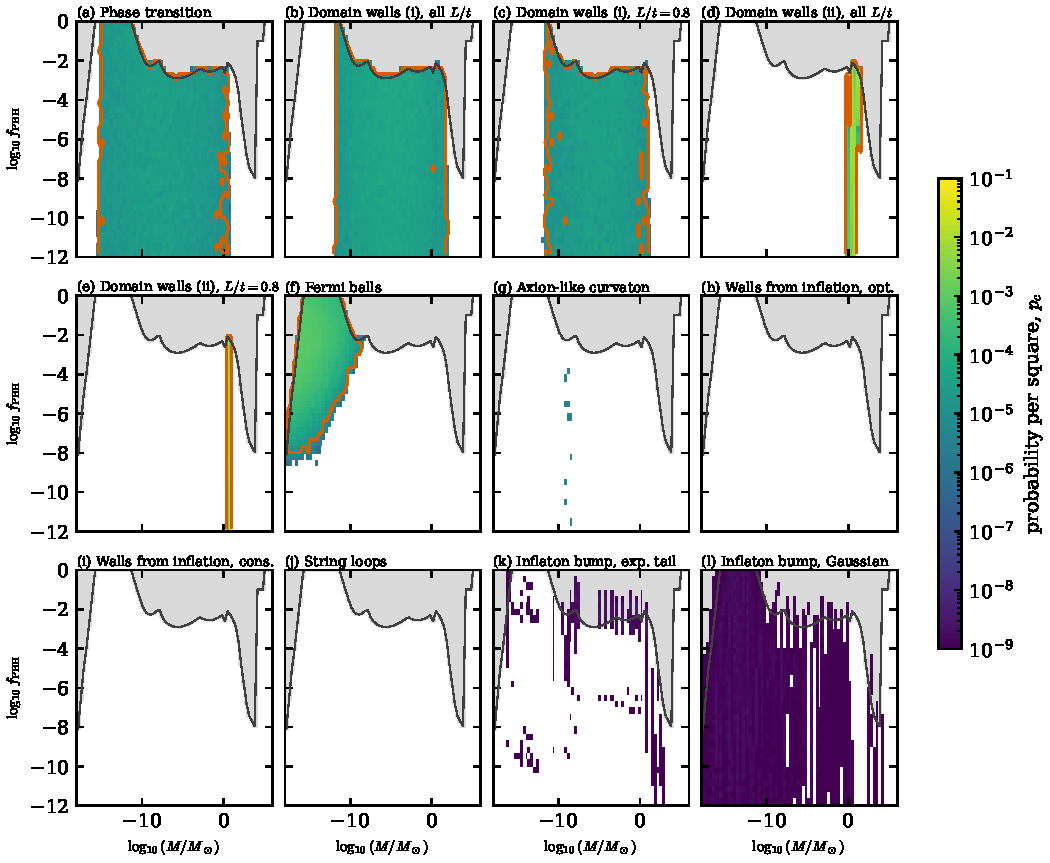
\includegraphics[width=\textwidth]{fig_individual_ref.pdf}
\caption{Per-mechanism maps on the reference inflation model, as they enter Fig.~2 of the paper: $p_c$ (maximum over the treatments indicated) and the contour $p_c=\epsilon$ (orange). (a) FOPT, non-covariant, $\delta_c=0.40$--$0.67$; (b),(c) domain walls, PTA case (i), all $L/t$ and $L/t=0.8$; (d),(e) the same for case (ii); (f) Fermi balls; (g) axion-like curvaton with the hilltop region counted; (h),(i) walls from inflation, $(A,\kappa)=(10^2,2)$ and $(10^{-2},1)$; (j) string loops with free collapse fraction; (k),(l) inflaton bump with exponential tail and Gaussian statistics. Panels (h)--(j) are empty because all samples within the limits lie at $\log_{10}(M/\Msun)\simeq-18.6$, below the plane. Grey: excluded by current limits.}
\label{fig:indref}
\end{figure*}

\begin{figure*}[htbp]
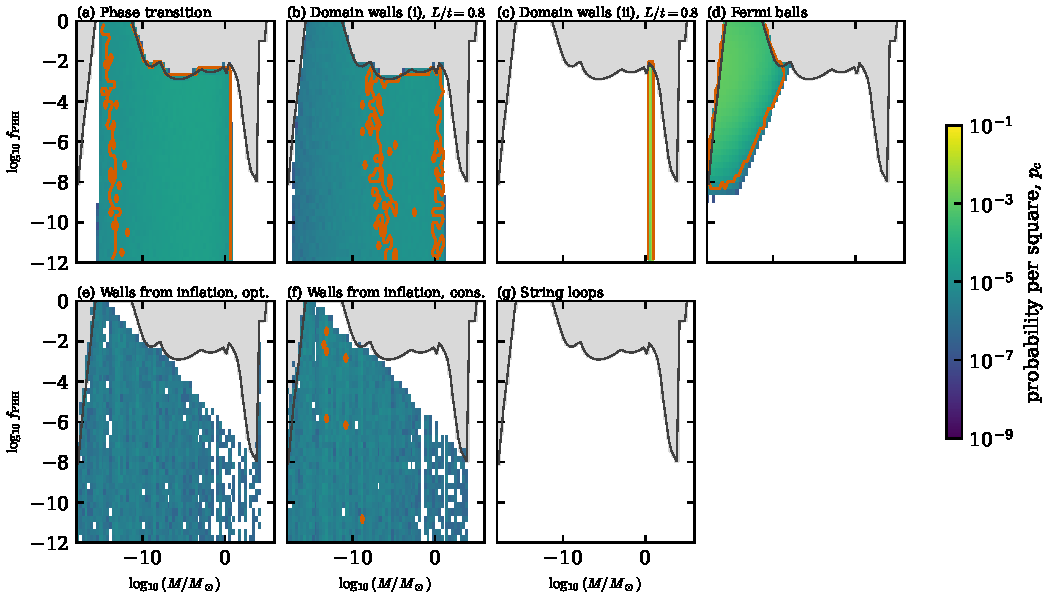
\includegraphics[width=\textwidth]{fig_individual_bg.pdf}
\caption{As Fig.~\ref{fig:indref} for the $\alpha$-attractor family of inflation models with free reheating (averaged over 480 inflation models). (a) FOPT; (b),(c) domain walls, cases (i) and (ii), $L/t=0.8$; (d) Fermi balls; (e),(f) walls from inflation, optimistic and conservative; (g) string loops.}
\label{fig:indbg}
\end{figure*}

%=======================================================================
\section{Analytic estimates and comparison with the numerical results}\label{sec:analytic}

Each estimate below uses leading-order formulas and, where a parameter distribution enters, the first two moments of the stored samples (\code{analytic.py}). Table~\ref{tab:analytic} compares them with the numerical results.

\subsection{Inflation models}

For plateau potentials $n_s\simeq1-2/\Ns$ and $r\simeq12\alpha/\Ns^2$. The exact slow-roll $n_s$ of the reference inflation model equals $1-2/(\Ns+2.05)$; we use this shift when converting $n_s$ bands to bounds on $\Ns$. With $H_\ast/H_{\rm end}\simeq1.5$, $\rho_{\rm end}\simeq0.43\,V_\ast$ and $V_\ast=\frac32\pi^2A_srM_P^4$,
\begin{equation}
\Ns\simeq\ln\frac{a_{\rm reh}H_{\rm reh}}{k_\ast}+\Big[\frac12-\frac1{3(1+\wreh)}\Big]\ln\frac{\rho_{\rm end}}{\rho_{\rm reh}}+\ln1.5,
\label{eq:Nan}
\end{equation}
which reproduces the exact $\Ns$ with an rms error of $0.35$ over the parameter range. The Planck band gives $\Ns\ge43.9$, the ACT band $\Ns\ge59.5$. Equation~\eqref{eq:Nan} gives $\Ns^{\max}=60.1$ at $\wreh=\frac12$ and $\Treh=5$\,MeV, so for $\alpha\lesssim1$ ACT is reachable only in a corner of the parameter range, as found numerically. For $\alpha\gtrsim8$ the relation $n_s\simeq1-2/\Ns$ no longer holds: the slow-roll $n_s$ at fixed $\Ns$ is larger, and the lower edge of the ACT band is also met at $\Ns=55$--$57$ with nearly instant reheating (Sec.~\ref{sec:infl}).

\subsection{Curvaton models}

\emph{Quadratic curvaton.} Using $r_\sigma\le\min(3p/4,1)$ and $\sigma_k\ge\sigma_{\rm end}$,
\begin{equation}
\mathcal{P}_\zeta(k_{\rm dec})\lesssim\frac49\,\frac{H_\ast^2}{24\pi^2M_P^2}\,\frac{\Treh}{T_{\rm dec}}\quad\text{(I)}.
\end{equation}
The CMB requirement $\mathcal{P}_\zeta(k_\ast)<0.01A_s$ and classicality $\mathcal{P}_x(k_{\rm end})<1$ for a constant decay rate $\lambda$ give, after maximizing over $\lambda$,
\begin{equation}
\mathcal{P}_\zeta(k)\lesssim0.01A_s\Big(\frac{4/9}{0.01A_s}\Big)^{\ln(k/k_\ast)/\Ns}\quad\text{(II)}.
\end{equation}
The minimum of (I) and (II) peaks at $1.8\times10^{-6}$ near $10^{-6}\,\Msun$. With $\Omega_{\rm dec}\to1$ and $\zeta_c=1$ the threshold is $x_c=e^{3/2}-1$, so $\log_{10}\beta\lesssim-x_c^2/(2\cdot\frac94\mathcal{P}_\zeta\ln10)\approx-6\times10^{5}$. The largest $\mathcal{P}_\zeta(k_{\rm dec})$ among allowed samples is $3.9\times10^{-9}$, below the bound.

\emph{Inflating curvaton.} At CMB scales $\zeta\simeq g_2^{-1}\delta\sigma/\sigma$ with $\delta\sigma=H_\ast/2\pi$, so $\mathcal{P}_\zeta(k_\ast)<0.01A_s$ requires
\begin{equation}
g_2\,\sigma_{\rm CMB}>\frac{H_\ast}{2\pi\,(0.01A_s)^{1/2}}=0.23\,M_P\,\frac{H_\ast}{1.6\times10^{13}\,{\rm GeV}},
\end{equation}
and $\sigma_{\rm CMB}<M_P$ gives $g_2>0.23$ on the reference inflation model, against $g_2>0.0035$ for $H_1=2.4\times10^{11}$\,GeV, the example of Ref.~\cite{Kohri:2012yw}. The allowed points have $g_2\ge0.25$. Reaching $\zeta_c$ then needs $|\ln|1+x||\ge g_2\zeta_c$ for $x=\delta\sigma/\sigma$ at the PBH scale, and the Gaussian tail gives $\log_{10}\beta\sim-(g_2\zeta_c)^2/(2\mathcal{P}_x\ln10)$. At the maximum of Sec.~\ref{sec:mech} ($g_2=0.62$) the largest $\mathcal{P}_x$ on PBH scales is $4.5\times10^{-6}$, which gives $-1.9\times10^{4}$, against $-3.8\times10^{3}$ numerically. The estimate uses $\mathcal{P}_x$ of a single scale, whereas the smoothed variance integrates it over several $e$-folds and is larger by a factor of about five; both values are far below any abundance of interest. Separately, $n_s(\Ns-N_2)\ge0.9565$ gives $N_2\le\Ns-46.0=5.0$ at leading order and $7.1$ with the shift, compared with $6.8$ from the exact solution.

\emph{Axion-like curvaton.} The total probability $3.7\times10^{-5}$ spread over the 10 squares it covers gives $3.7\times10^{-6}$ per square on average; the largest square has $6.7\times10^{-6}<\epsilon$. With $10^{6}$ samples and the PBH limits, lowering the threshold to $\zeta_c=0.5$ raises the total thirteenfold, from $2.7\times10^{-5}$ to $3.6\times10^{-4}$, but the number of squares covered grows from 23 to 196, so the mean per square stays at $(1$--$2)\times10^{-6}$ and the largest square has $8\times10^{-6}$.

\subsection{FOPT}

Since $\log\fpbh$ is linear in $\log T_{\rm eq}$ and steep in $b=\beta/H$, the abundance lies in $(10^{-12},1)$ only in a narrow interval of $b$ at each temperature, centred on $b_\ast\simeq6.1$ ($\delta_c=0.5$). Integrating the conditional Gaussian of $b$ over this interval gives
\begin{equation}
P(10^{-12}<\fpbh<1)=\int d\log T\,\pi(\log T)\int_{b_1(T)}^{b_2(T)}db\,\pi(b|\log T),
\end{equation}
$0.020$ against $0.028$ numerically: the bimodality is a property of the map, not of the sampling. With the covariance scaled by $s^2$ the same formula gives $0.0004$ ($s=0.5$) and $0.026$ ($s=2$), against $0.0025$ and $0.042$ from the reruns. It explains why halving the spread of the parameter distribution removes most of the FOPT reach (Sec.~VI of the paper); the residual factor reflects the non-Gaussian tails of the distribution cut off at the edge of $R$.

The light edge follows from LVK. Above the peak $S_{\rm env}\simeq1.357f_{\rm env}/f$, so $\Omega(20\,{\rm Hz})<5.8\times10^{-9}$ requires $f_{\rm env}$ below a temperature-dependent value; at $b_\ast$ this gives $T_{\rm eq}\lesssim10^{6.7}$\,GeV and $\log_{10}(M/\Msun)\gtrsim-15.4$. The heavy edge follows from the PTA band: below the peak $S_{\rm env}\simeq3.8(f/f_{\rm env})^{2.8}$, and requiring $\Omega(30\,{\rm nHz})$ below the signal amplitude gives $T_{\rm eq}\gtrsim0.45$\,GeV, $\log_{10}(M/\Msun)\lesssim-1.2$. A pointwise PTA limit gave $-0.6$ numerically; the likelihood, which lets the FOPT spectrum share the signal with the SMBHB background, extends the edge to $+0.2$. The same temperature, $T_{\rm eq}\simeq0.45$\,GeV, sets the reheating temperature below which the FOPT cannot reach the window (numerically $\sim0.1$\,GeV).

\subsection{Domain walls}

Walls form after reheating if $\sigma^{1/3}<\Treh$ with $\sigma=3\alpha_{\rm ann}M_P^2/(4\mathcal{A}t_{\rm ann})$ and $t_{\rm ann}=1/2H(T_{\rm ann})$, i.e.\ $\sigma^{1/3}\sim(\alpha_{\rm ann}M_PT_{\rm ann}^2)^{1/3}$; at the NG15 best fit this is $10^{5.4}$\,GeV. The monochromatic mass $M=4\pi M_P^2t_{\rm ann}/\sqrt{3\alpha_{\rm ann}}$ is $10^{0.74}\,\Msun$ at the best fit and spans $10^{0.1}$--$10^{1.6}\,\Msun$ over the NG15 band; the critical-collapse width shifts the peak down by $0.1$--$0.2$\,dex (Sec.~\ref{sec:dw}). In case (i), eliminating $t_{\rm ann}$ gives $M\simeq\pi\sqrt{3\alpha_{\rm ann}}M_P^4/(\mathcal{A}\sigma)$, so $\sigma^{1/3}<\Treh$ sets the light edge at $10^{-11.4}$--$10^{-10.9}\,\Msun$ for $\alpha_{\rm ann}=0.1$--$1$. The heavy end of the NG15 band, $10^{1.6}\,\Msun$, bounds the domain-wall band that is reached in every variation in scenarios (c) and (d).

\subsection{Fermi balls}

Both $\log M$ and $\log\fpbh$ are linear in $\theta=(\log T_\ast,\log\beta/H,\log\alpha,\log\eta_\chi)$ at fixed $g_\ast$:
\begin{align}
\log M&=c_M-2\log T_\ast-3\log\tfrac{\beta}{H}+\tfrac14\log\alpha+\log\eta_\chi,\\
\log\fpbh&=c_f+\log T_\ast+\tfrac14\log\alpha+\log\eta_\chi,
\end{align}
so a Gaussian parameter distribution is mapped to a bivariate Gaussian with mean $A\mu$ and covariance $A\Sigma A^{\rm T}$. With $g_\ast=10$ this gives $\langle\log M\rangle=-21.8$, $\sigma_{\log M}=5.1$, $\langle\log\fpbh\rangle=-2.0$, $\sigma_{\log f}=1.75$, correlation $-0.17$, and an evaporated fraction $\Phi[(\log M_{\rm ev}-\langle\log M\rangle)/\sigma_{\log M}]=0.735$, against $0.731$ numerically. The lower boundary of the reach in the asteroid-mass window (Sec.~IV\,D of the paper) is a contour of constant density of this Gaussian.

\subsection{Walls from inflation and string loops}

For $\psi\propto M^{-1/2}$ the abundance sits at the lightest surviving mass, $\max[M_{\rm ev},M_H(\Treh)]$. On the reference inflation model this is $M_{\rm ev}$, $\log_{10}(M/\Msun)=-18.59$, as found. The peak enters the plane when $M_H(\Treh)=4.8\times10^{-2}\Msun({\rm GeV}/\Treh)^2>10^{-18}\Msun$, i.e.\ $\Treh<10^{8.3}$\,GeV. The median of $M_H(\Treh)$ over the distribution of inflation models restricted to this range is $10^{-10.4}\,\Msun$, against the numerical median $10^{-11.6}\,\Msun$ of the reach, which weights low-$\Treh$ inflation models by their larger reach. At the lowest reheating temperature, 5\,MeV, $M_H(\Treh)=2\times10^{3}\,\Msun$, the heaviest mass that walls from inflation produce in the family.

For strings, integrating $\psi$ above $M_{\rm ev}$ gives $\fpbh^{\rm tot}=(c_s/\Omega_{\rm DM})(M_{\rm ev}/M_\ast)^{-1/2}$, so the evaporated-PBH limit $c_s<6.3\times10^{-11}$ implies $\fpbh^{\rm tot}<2.4\times10^{-10}$. Requiring $\fpbh^{\rm tot}>10^{-12}$ with $f\le1$ needs $G\mu\gtrsim2\times10^{-21}$, i.e.\ $\eta\gtrsim2\times10^{8}$\,GeV; with $T_{\max}\propto\Treh^{1/2}$ this requires $\Treh\gtrsim10^{1.5}$\,GeV, compared with the numerical transition at $10^{2}$--$10^{4}$\,GeV.

\subsection{Inflaton bump}

Near $A_c$ the peak power scales as $\mathcal{P}_{\max}\simeq K\delta^{-2}$ with $K\simeq3\times10^{-10}$ (median over nodes), and $\ln\beta\propto-1/\mathcal{P}_{\max}\propto-\delta^2$. Between $\fpbh=1$ (at $\delta_0$, with $|\ln\beta_0|\simeq34$) and $\fpbh=10^{-12}$ the shell therefore has
\begin{equation}
\Delta\ln A\simeq\delta_0\Big[\Big(1+\frac{12\ln10}{|\ln\beta_0|}\Big)^{1/2}-1\Big],
\end{equation}
$4.9\times10^{-5}$ against $5.1\times10^{-5}$ from the scans (medians over the 55 nodes of the coarse grid, Gaussian statistics). The probability of the shell is the allowed fraction ($0.47$) times the probability density of $\log A$ at $A_c$ times $\Delta\log A$, $1.0\times10^{-6}$ against $2.4\times10^{-6}$; spread over $\gtrsim10^2$ squares, this is far below $\epsilon$ per square.

\subsection{A Gaussian model of the reached region}

The reach of a treatment can be modelled by replacing its samples within the limits by a bivariate Gaussian in $(\log M,\log\fpbh)$ with their mean $m$, covariance $C$ and total probability $P$. Then $p_c=PN(x_c;m,C)/9$ and the reached region is an ellipse of area (in squares)
\begin{equation}
\mathcal{A}=2\pi\cdot9\,\sqrt{|C|}\,\ln\frac{P}{18\pi\sqrt{|C|}\,\epsilon},
\label{eq:ellipse}
\end{equation}
which vanishes for $\epsilon>P/(18\pi\sqrt{|C|})$. Equation~\eqref{eq:ellipse} explains the threshold curves of Fig.~3 of the paper: the FOPT and domain walls (case i) spread $P\sim0.03$ over $\sim10^3$ squares, so their peak $p_c$ is a few $\times10^{-5}$ and their area collapses between $\epsilon=10^{-5}$ and $10^{-4}$, while Fermi balls ($P=0.18$ concentrated near the limits) and domain walls in case (ii) ($P=0.4$ in a narrow band) keep their reach. A spread scaling $C\to s^2C$ at fixed $P$ lowers the peak density by $s^{-2}$ for $s>1$ and raises it for $s<1$; at the same time $P$ itself changes for mechanisms with a bimodal abundance, which this model does not capture.

Table~\ref{tab:analytic} compares the model with the numerical maps. It reproduces the (A) fractions at $\epsilon=10^{-6}$ and $10^{-4}$ to within $0.11$ and the per-mechanism areas of Fermi balls and domain walls (case ii) to within 10\%. At $\epsilon=10^{-5}$ it underestimates the FOPT and domain-wall (case i) areas by 25--40\% because their mass distributions are flatter than Gaussian, and it fails for spread variations where $P$ changes. These failures identify where the numerical treatment is indispensable.

\begin{table*}[htbp]
\caption{Analytic estimates (Sec.~\ref{sec:analytic}) and numerical results. Masses in $\log_{10}(M/\Msun)$, temperatures in $\log_{10}(T/{\rm GeV})$. Scenarios (a)--(d) as in Table~III of the paper.}
\label{tab:analytic}
\small
\begin{ruledtabular}
\begin{tabular}{lll}
Quantity & Analytic & Numerical \\
\hline
Reference $n_s$; $r$ & $0.9608$; $0.0046$ & $0.9623$; $0.0040$ \\
$\Ns$ over the $\alpha$-attractor range, rms (max) error & --- & $0.35$ ($1.2$) \\
Achievable $\Ns$ range ($\alpha=1$) & $42.1$--$60.1$ & $41.4$--$62.4$ (all $\alpha$) \\
Lowest $\Ns$ allowed by Planck & $43.9$ & $43.8$ \\
$\log\alpha_{\max}$ from $r<0.036$ & $1.0$ & $1.3$ \\
Quadratic curvaton $\max\mathcal{P}_\zeta(k_{\rm dec})$ & $\le1.8\times10^{-6}$ & $3.9\times10^{-9}$ \\
Inflating curvaton $g_2^{\min}$; $\max\log_{10}\fpbh$ & $0.23$; $\sim-1.9\times10^{4}$ & $0.25$; $-3.8\times10^{3}$ \\
Inflating curvaton $N_2^{\max}$ & $5.0$ / $7.1$ (shifted) & $6.8$ \\
Axion-like curvaton mean / max $p_c$ & $3.7\times10^{-6}$ & $6.7\times10^{-6}$ \\
\quad same, $\zeta_c=0.5$ ($10^6$ samples) & $1.8\times10^{-6}$ & $8\times10^{-6}$ \\
FOPT $P(10^{-12}<\fpbh<1)$; spread $\times0.5$; $\times2$ & $0.020$; $0.0004$; $0.026$ & $0.028$; $0.0025$; $0.042$ \\
FOPT light edge (LVK) & $-15.4$ & $-15.2$ \\
FOPT heavy edge & $-1.2$ (pointwise) & $-0.6$ (pointwise); $+0.2$ (likelihood) \\
FOPT minimal $\Treh$ & $-0.35$ & $\sim-0.9$ \\
DW minimal $\Treh$ & $5.4$ & $5.2$ \\
DW mass at NG15 best fit; band & $0.74$; $0.1$--$1.6$ & $0.77$; $-0.1$--$1.4$ \\
DW light edge, case (i) & $-11.4$ to $-10.9$ & $-11.5$ \\
Fermi balls $\langle\log M\rangle$, $\sigma$ & $-21.8$, $5.1$ & $-22.0$, $5.1$ \\
Fermi balls $\langle\log f\rangle$, $\sigma$; correlation & $-2.0$, $1.75$; $-0.17$ & $-1.85$, $1.79$; $-0.20$ \\
Fermi balls evaporated fraction & $0.735$ & $0.731$ \\
Walls: peak mass (ref.); $\Treh$ of entry into the plane & $-18.59$; $8.3$ & $-18.59$; $\sim8$ \\
Walls: median mass (family of inflation models) & $-10.4$ & $-11.6$ \\
Strings: $\fpbh^{\rm tot,max}$; minimal $\Treh$ & $2.4\times10^{-10}$; $1.5$ & $2.5\times10^{-10}$; $2$--$4$ \\
Inflaton bump $\Delta\ln A$; $P(10^{-12}<f<1)$ & $4.9\times10^{-5}$; $1.0\times10^{-6}$ & $5.1\times10^{-5}$; $2.4\times10^{-6}$ \\
(A) fraction, $\epsilon=10^{-6}$, (a)--(d) & $0.11, 0.18, 0.17, 0.74$ & $0.19, 0.29, 0.21, 0.76$ \\
(A) fraction, $\epsilon=10^{-5}$, (a)--(d) & $0.31, 0.43, 0.41, 0.79$ & $0.20, 0.33, 0.22, 0.78$ \\
(A) fraction, $\epsilon=10^{-4}$, (a)--(d) & $0.88, 0.88, 0.84, 0.85$ & $0.87, 0.87, 0.81, 0.84$ \\
(A) fraction, spread $\times0.5$, (a)--(d) & $0.55, 0.72, 0.62, 0.89$ & $0.53, 0.71, 0.80, 0.86$ \\
(A) fraction, spread $\times2$, (a)--(d) & $0.17, 0.42, 0.57, 0.59$ & $0.20, 0.30, 0.21, 0.76$ \\
Reached squares, $\epsilon=10^{-6},10^{-5},10^{-4}$: FOPT & $1608, 736, 0$ & $1465, 1238, 0$ \\
\quad DW (i), $L/t=0.8$ & $1428, 802, 0$ & $1117, 1049, 0$ \\
\quad Fermi balls & $493, 381, 254$ & $450, 399, 280$ \\
\quad DW (ii), $L/t=0.8$ & $59, 59, 57$ & $59, 59, 59$ \\
\end{tabular}
\end{ruledtabular}
\end{table*}

%=======================================================================
\section{Reproducing the results}\label{sec:repro}

\paragraph*{Setup.}
Python 3.10 or later with numpy $\ge2.0$, scipy and matplotlib (\code{requirements.txt}). The external data of Table~\ref{tab:inputs} are placed in \code{external/} (PBHbounds, ceffyl data, the NANOGrav 15-year KDE files); \code{setup.ps1} or \code{setup.sh} creates the environment and checks the data. The number of parallel processes is set with \code{PBH\_NPROC}.

\paragraph*{Main results.}
From \code{pbh/}, \code{python regenerate.py} rebuilds the stored results of the reference analysis in the order listed at the top of that file and compares them with the values in \code{expected/}; \code{--full} also repeats the slow scans (inflaton bump, walls from inflation, strings). On an 8-core desktop the standard run takes 1.5--2.5 hours.

\paragraph*{Additional steps.}
The following are run separately, in this order, after the main results:
\begin{enumerate}
\item fine grid of bump positions: \code{PBH\_USR\_DPHI=0.025 PBH\_USR\_NODES=usr\_nodes\_fine.npy python usr\_pipeline.py}, then \code{PBH\_USR\_TAG=\_fine PBH\_USR\_NODES=usr\_nodes\_fine.npy python usr\_pushforward.py} (about 4 hours with 10 processes);
\item family of inflation models: \code{python bg\_prior.py}, \code{python bg\_run.py planck 20000}, \code{python bg\_combine.py};
\item variations: \code{python robustness.py run}, \code{PBH\_MEASURE=flat} runs of \code{bg\_node.py} (files \code{bgscan/robust/flat.npz} and \code{flatwide.npz}, the latter with \code{PBH\_BOXVAR=wide}), then \code{python robustness.py analyze};
\item ACT-compatible inflation models: \code{python bg\_prior\_act.py 60}, \code{PBH\_BGPRIOR=bg\_prior\_act.npz python bg\_run.py actH 50000} and the same for \code{actL}, then \code{python bg\_act\_combine.py};
\item maps and threshold curves: \code{python measure\_checks.py}, \code{python measure\_plots.py};
\item checks of Sec.~IV of the paper: \code{infcurv\_opt\_de.py}, \code{axion\_zc.py}, \code{axion\_target\_de.py}, \code{fopt\_gwvar.py run} for \code{env}, \code{LV3}, \code{LV2} followed by \code{fopt\_gwvar.py analyze}, \code{dw\_bayes.py}, \code{infwall\_reh.py};
\item figures of the paper: \code{python fig\_combined.py}, \code{python paper\_figs.py}.
\end{enumerate}
The stored samples of all results take about 5\,GB.

\bibliography{refs}

\end{document}
